\documentclass[11pt]{beamer}
\usetheme{Copenhagen}
\usepackage[utf8]{inputenc}
\usepackage{hyperref}
\usepackage{amsmath}
\usepackage{amsfonts}
\usepackage{amssymb}
\usepackage{graphicx}
\usepackage{xcolor}
\usepackage{tikz}
\usetikzlibrary{shapes, arrows, calc, arrows.meta, fit, positioning} % these are the parameters passed to the library to create the node graphs  
\tikzset{  
    -Latex,auto,node distance =1.5 cm and 1.3 cm, thick,% node distance is the distance between one node to other, where 1.5cm is the length of the edge between the nodes  
    state/.style ={ellipse, draw, minimum width = 0.9 cm}, % the minimum width is the width of the ellipse, which is the size of the shape of vertex in the node graph  
    point/.style = {circle, draw, inner sep=0.18cm, fill, node contents={}},  
    bidirected/.style={Latex-Latex,dashed}, % it is the edge having two directions  
    el/.style = {inner sep=2.5pt, align=right, sloped}  
}  

\usepackage[backend=bibtex,style=ieee]{biblatex}
\addbibresource{group_protocols_auth.bib}

\setbeamertemplate{frametitle continuation}{}

\author{Andrei Cristian\\
\href{mailto:andrei.cristian1@info.uaic.ro}{andrei.cristian1@info.uaic.ro}}
\title{Verificarea protocoalelor de autentificare de grup prin Scyther}
\setbeamercovered{transparent} 
\setbeamertemplate{navigation symbols}{} 
%\logo{} 
%\institute{} 
\date{\today} 
%\subject{} 
\begin{document}

\begin{frame}
\titlepage
\end{frame}

\begin{frame}
\tableofcontents
\end{frame}

\section{Introducere}

\begin{frame}{Introducere}

Lucrarea "Verifying Group Authentication Protocols by Scyther", Huihui Yang, Vladimir Oleshchuk, and Andreas Prinz(University of Agder, Kristiansand, Norway) prezinta analiza a doua protocoale complexe de autentificare de grup folosind Scyther.

Din cauza limitarii utilitarului, doar un subset de proprietati de securitate au fost verificate:
\begin{itemize}
\item autentificare mutuala;
\item autentificare cu cheie implicita \footnote{proprietatea in care una dintre parti este asigurata ca nicio alta parte in afara de o a doua parte identificata in mod specific nu poate avea acces la o anumita cheie secreta};
\item siguranta impotriva atacurilor de impersonare si adversarilor pasivi.
\end{itemize}

\end{frame}

\begin{frame}{Scyther}
\begin {itemize}
\item Pentru verificarea securitatii protocoalelor exista doua abordari principale: securitatea demonstrabila (eng. \textit{provable security}) si metodele formale (eng. \textit{formal methods}).
\item \textbf{Scyther} este un utilitar de verificare formala si este conceput pentru verificarea automata a protocoalelor de securitate.
\item Modelul adversarial este predefinit si anume modelul Dolev-Yao. Aceasta abordare simplifica formalizarea protocoalelor de securitate si il face mai usor de folosit pentru utilizatorii noi.
\item Poate oferi clase de comportament de protocol spre deosebire de doar urmele de atac (furnizate in cazul altor utilitare).

\end{itemize}
\end{frame}

\begin{frame}{Protocoale de autentificare de grup}

\begin{itemize}
\item Scopul principal este imbunatatirea eficientei autentificarii pentru grupuri mari
\item Relatia dintre autentificator si utilizatorii care urmeaza sa fie autentificati este unu la unu.
\item In acest tip de protocol de autentificare de grup, autentificatorul \textbf{poate autentifica mai multi utilizatori in acelasi timp}.
\item Daca in protocol autentificarea are acces:
\begin{itemize}
	\item autentificarea mutuala ar trebui sa fie satisfacuta;
	\item se va stabili o cheie de sesiune de grup.
\end{itemize}
\end{itemize}

\end{frame}

\begin{frame}{Ce urmareste lucrarea}

\begin{itemize}

\item Extinderea lucrarii \cite{fagrauth};
\item In lucrarea mentionata, marimea grupului era de 3, iar in aceasta lucrare sunt analizate cazurile pentru grupuri ce contin doi, trei si patru membri.
\item Formalizarea protocoalele bazate pe DLP\footnote{discrete logharitm problem} de tipurile I si II (tip II = autentificatorul are certificat bazat pe PKI\footnote{public key infrastructure}; tip I = autentificatorul nu are certificat) cand numarul de membri din grup este $N(N\geq3)$.
\item Analiza unor noi proprietati ale protocoalelor, precum "Alive" si "Nisynch"

\end{itemize}

\end{frame}

\section{Descrierea protocoalelor de autentificare de grup}
\begin{enumerate}
\begin{frame}{Scenarii de utilizare}

\item \begin{itemize}
	\item Asa cum este prezentat in figura \ref{fig:type1use}, autentificatorul de tip I are o lista de prieteni, dar membrii din aceasta lista se pot sau nu cunoaste intre ei.
	\item De fiecare data inainte de intalnirea grupului, autentificatorul intai selecteaza membrii grupului si apoi trebuie sa autentifice fiecare membru din acest grup.
	\item Cum toti membrii s-au inregistrat deja ca prieteni ai autentificatorului, presupunem ca acestia partajeaza niste secrete cu autentificatorul inainte de autentificare.
	\end{itemize}

\end{frame}

\begin{frame}{Scenariul de utilizare pentru protocoale de tip I}

\begin{figure}\label{fig:type1use}
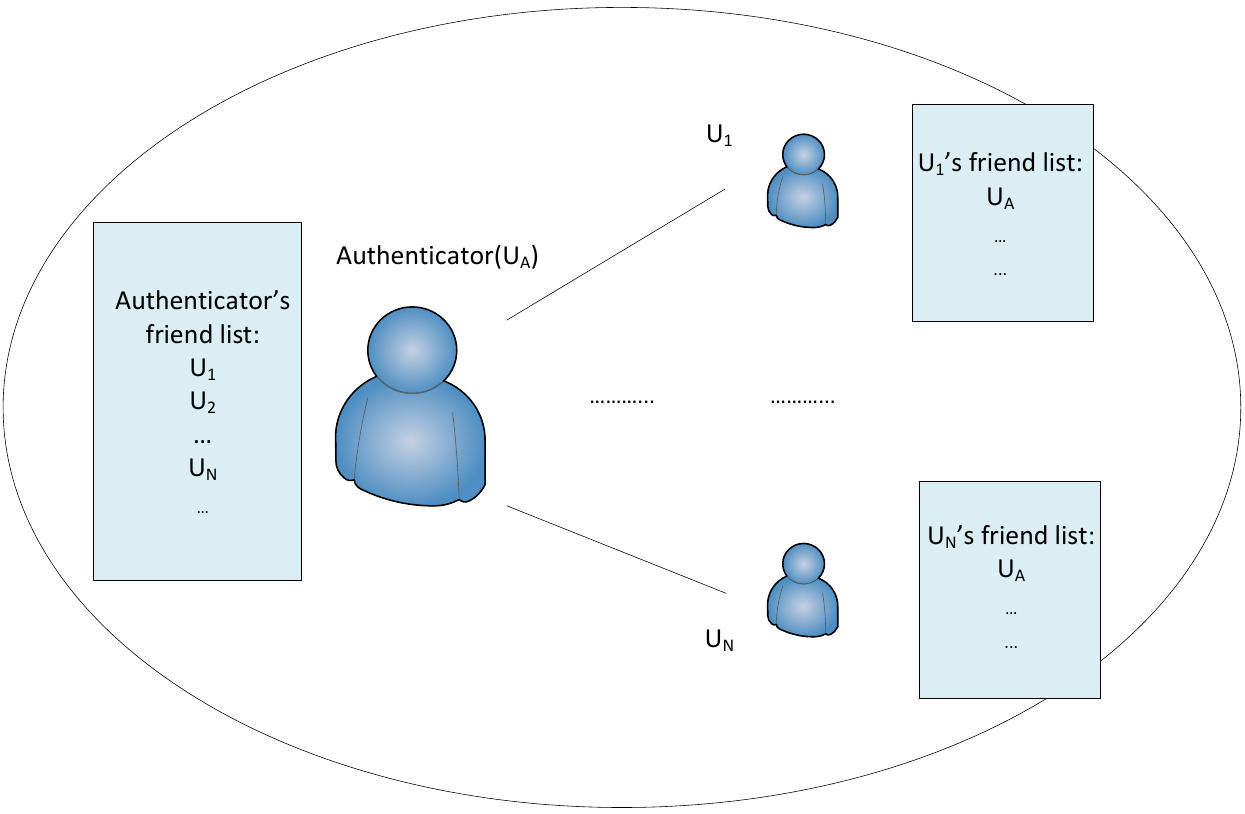
\includegraphics[scale=0.25]{type1_use.png} 
\caption{Scenariul de utilizare 1: Tipul I}
\end{figure}

\end{frame}

\begin{frame}{Scenarii de utilizare}

\item \begin{itemize}

	\item In protocoalele de tip II (figura \ref{fig:type2use}), autentificatorul este un server.
	\item Trebuie sa autentifice utilizatori pe care nu ii cunoaste neaparat dinainte.
	\item In acest caz, serverul trebuie sa detina un certificat pentru a realiza autentificarea grupului.

\end{itemize}

\end{frame}

\begin{frame}{Scenariul de utilizare pentru protocoale de tip II}

\begin{figure}\label{fig:type2use}
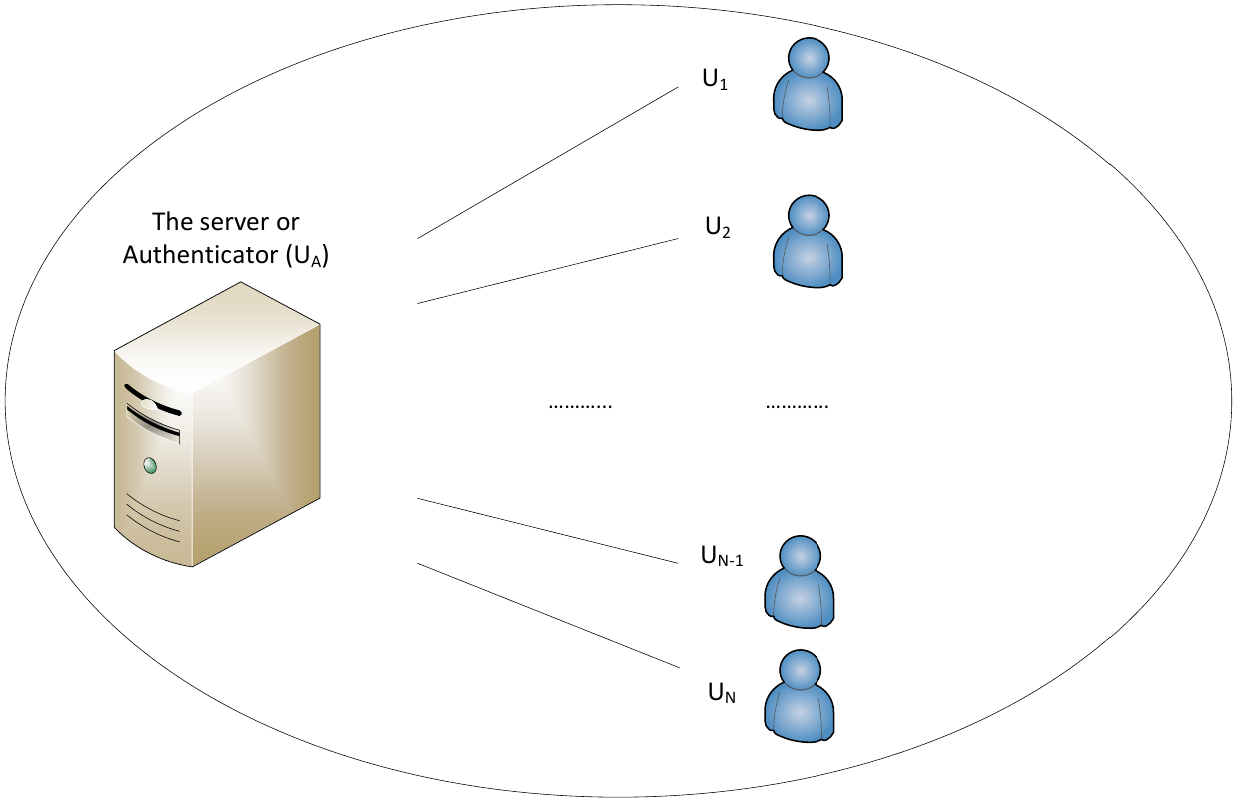
\includegraphics[scale=0.25]{type2_use.png} 
\caption{Scenariul de utilizare 2: Tipul II}
\end{figure}

\end{frame}

\end{enumerate}

\begin{frame}{Un framework general}

Presupunem ca sunt $N$ membri in grupul de utilizatori $\mathbb{U}$. Fluxul de mesaje al frameworkului general propus in \cite{generalframework} poate fi descris in urmatorii patru pasi:
\begin{enumerate}

\item $U_A \rightarrow U_1: ID_A, UID, X, C_0, MAC_A$.

\item $U_i \rightarrow U_{i+1}: ID_i, UID, X, KP_U, C_i, MAC_i$, unde $1 \leq i \leq N - 1$.

\item $U_N \rightarrow U_A: ID_N, KP_U, C_N, MAC_N$.

\item $U_A \rightarrow \mathbb{U}: Y, MAC'_A$.

\end{enumerate}
Pentru $j \in \{A,N,U_i\}$, 
$ID_j$ este identitatea lui j, $UID$ este setul de identitati al tuturor utilizatorilor din $\mathbb{U}$, $X$ este o informatie importanta pe care $U_A$ vrea sa o transmita la tot grupul, $C_k$ este utilizat pentru a calcula $C_{k+1}$, pt. $k=0..N-1$, $MAC_j$ este codul de autentificare al mesajului, $KP_U$ este setul de parametri cheie al grupului de utilizatori $\mathbb{U}$, iar Y contine parametrii cheie generati de $\mathbb{U}$.

\end{frame}

\begin{frame}[t,allowframebreaks]{Protocoale bazate pe problema logaritmului discret}
Calcularea parametrilor $C_i (0 \leq i \leq N)$, $X$ si $Y$ ai protocolului bazat pe DLP pentru ambele tipuri Tipul I si Tipul II.

\begin{enumerate}

\item $C_0$ este calculat de catre $U_A$ prin $C_0 = \xi(r) = \xi(g^r_A)$, unde $r_A \in [1, p-1]$ este un numar generat aleator, $\xi$ este un mesaj ce va fi criptat prin algoritmul de criptare Elgamal. Similar, $U_i (2 \leq i \leq N)$ calculeaza $C_i = C_{i-1} \times r^{x_i} = \xi(r^{\sum^i_{t=1}x_t})$.

\item $X$ este calculat ca solutie a $X \equiv V_i$ mod $k_i (1 \leq  i \leq N)$, folosind teorema chineza a resturilor (CRT), unde $k_i$ este un secret partajat intre $U_A$ si $U_i$.

\begin{itemize}

\item Tipul I: $V_i = \{y_i \oplus K_G, y_i \oplus t_i, g^{m_i}, h_i\}$, iar $h_i = H(ID_A \oplus ID_i \oplus y_A \oplus t_i)$ si este folosit pentru autentificarea lui $U_A$ cu $U_i$. Aici, $y_i$ este un secret predistribuit intre $U_A$ si $U_i$, $K_G$ este cheia de sesiune a grupului generata de $U_A$, $t_i$ este un nonce si $g^{m_i}$ este parametrul cheie generat de $U_A$ pentru a calcula cheia partajata intre $U_A$ si $U_i$.
\item Tipul II: $V_i = SIGN_{SK_A}\{ID_A, ID_i, K_G, G^{m_i}, t_i\}$. Parametrii $g^{m_i}$ si $t_i$ au aceeasi semnificatie ca in cazul Tipului I. Autentificarea lui $U_A$ este realizata prin verificarea folosind semnatura sa in loc de utilizarea lui $h_i$ ca in cazul Tipului I.

\end{itemize}

\item $U_A$ calculeaza $Y$ prin rezolvarea $Y \equiv W_i$ mod $k_i (1 \leq i \leq N)$, unde $W_i = \{ID_A, ID_i, KP_i\}$ si $KP_i = KP_U - \{G^{n_i}\}$.

\item Cheia sesiunii dintre $U_A$ si $U_I$ este calculata ca find  $g^{m_in_j}$, in timp ce cheia sesiunii dintre $U_i$ si $U_j$ $(1 \leq i, j \leq N, i \neq j)$ este calculata ca fiind $g^{n_in_j}$.

\end{enumerate}

\end{frame}

\section{Utilitarul Scyther}
\subsection{Modelul adversarului in Scyther}

\begin{frame}[t,allowframebreaks]{Modelul adversarului in Scyther}
\begin{itemize}

\item Modelul adversarului in Scyther este predefinit si se bazeaza pe modelul \textit{Dolev-Yao} \cite{dolevyao}.

\item Nu trebuia sa formalizam abilitatile adversarului cand analizam protocoale.

\item Adversarul (notat cu \textbf{A}) poate \textbf{intercepta mesaje} de pe canalul de comunicare si poate \textbf{invata} din mesajele pe care le are.

\item Presupunem ca $M$ este setul de cunostinte al adversarului si $f$ este o functie prin care se exprima relatiile intre diferite elemente din M.

\item k poate reprezenta atat o cheie simetrica, dar si asimetrica, iar $k^{-1}$ este inversul acesteia ($k^{-1}=k$ in cazul cheii simetrice).

\item Fie $(t_i,t_j)$ reprezentarea concatenarii intre termenii $t_i$ si $t_j$.

\begin{itemize}

	\item $t \in M \Rightarrow M \vdash t$: daca \textit{t} este un element al lui \textit{M}, atunci \textit{A} cunoaste \textit{t}.
	\item $M \vdash (t_1, t_2) \Rightarrow \{ M \vdash t_1, M \vdash t_2 \}$: daca \textit{A} cunoaste $(t_1, t_2)$, atunci \textit{A} cunoaste ambii termeni $t_1$ si $t_2$.
	\item $\{ M \vdash t_1, M \vdash t_2 \} \Rightarrow M \vdash (t_1, t_2)$: daca \textit{A} cunoaste ambii termeni $t_1$ si $t_2$, atunci A cunoaste $(t_1, t_2)$.
	\item $\wedge_{1 \leq i \leq n} M \vdash t_i \Rightarrow M \vdash f(t_1, ..., t_n)$: daca \textit{A} cunoaste toti $t_i (1 \leq i \leq n )$ si \textit{f} este o functie publica, atunci \textit{A} poate calcula rezultatul functiei \textit{f} cu datele de intrare $t_1, ..., t_n$.
	\item $\{ M \vdash t, M \vdash k \} \Rightarrow M \vdash \{ t \}_k$: daca \textit{A} cunoaste mesajul \textit{t} si cheia \textit{k}, atunci A poate calcula mesajul criptat $\{ t \}_k$.
	\item $\{ M \vdash \{ t \}_k, M \vdash k^{-1} \} \Rightarrow M \vdash t$: daca \textit{A} cnoaste mesajul criptat $\{ t \}_k$ si cheia de decriptare $k^{-1}$, atunci \textit{A} poate decripta criptotextul si obtine astfel plaintextul \textit{t}.

\end{itemize}

\item In plus, adversarul A poate sa stearga, sa creeze noi mesaje si sa le insereze in canalul de comunicare.

\end{itemize}

\end{frame}

\subsection{Specificarea cerintelor de securitate in Scyther}
\begin{frame}[t,allowframebreaks]{Specificarea cerintelor de securitate in Scyther}

\begin{itemize}

\item Evenimentul \textbf{match} poate fi folosit in doua moduri diferite:

	\begin{enumerate}

	\item Specificarea constrangerilor de egalitate - de exemplu codurile dupa evenimentul $match(p_1, p_2)$ pot fi executate doar daca $p_1$ este egal cu $p_2$.
	\item Asemanator cu `=` din limbajul de programare \textbf{C}, daca \textit{p} este o variabila, iar \textit{v} este o valoare, atunci $match(p, v)$ semnifica asignarea valorii \textit{v} variabilei \textit{p}.
	
	\end{enumerate}
	
\item \textbf{claim} este folosit pentru specificarea cerintelor de securitate \textbf{Alive, Nisynch, secret} si \textbf{commitment}.
	\begin{itemize}

	\item \textbf{Alive} este o forma de autentificare care are ca scop asigurarea ca intr-adevar partea de comunicare destinata (R) a executat niste evenimente - $claim(R,\textbf{Alive})$.
	
	\item \textbf{Nisynch} semnifica faptul ca toate mesajele primite de R sunt intr-adevar trimise de catre partenerul de comunicare (sender) si au fost primite de carte celalalt partener de comunicare (receiver) - $claim(R,\textbf{Nisynch})$.
	
	\item $claim(R, \textbf{secret}, rt)$ inseamna ca R pretinde ca termenul \textit{rt} sa nu fie stiut de catre adversar.
	
	\item daca \textit{rt} este o cheie de sesiune, folosim $claim(R,\textbf{SKR}, rt)$ pentru a specifica acest lucru.
	
	\item \textbf{Commitment} este o promisiune a unei parti din comunicare catre alta parte. De exemplu, $claim(R,\textbf{Commit}, R', t)$ inseamna ca rolul \textit{R} face o promisiune \textit{t} catre rolul \textit{R'}. \textbf{Commitment} este folosit pentru a verifica protocoalele impotriva \textbf{atacurilor de uzurpare} (en. impersonation attacks).
	
	\end{itemize}

\end{itemize}

\end{frame}

\section{Analiza formala a protocoalelor de Tip I}

\subsection{Formalizarea cerintelor de securitate}

\begin{frame}[t,allowframebreaks]{Formalizarea cerintelor de securitate}

Fie \textit{R} si \textit{R'} doua parti de comunicare. Se pretinde ca protocoalele bazate pe problema logaritmului discret indeplinesc urmatoarele cerinte de securitate:

\begin{enumerate}

\item \textbf{Autentificarea mutuala}

	\begin{itemize}

	\item Autentificarea este calea prin care asiguram o parte a comunicarii ca aceasta comunica intr-adevar cu partea dorita. Daca autentificarea este indeplinita de ambele parti ale comunicarii, aceasta se numeste \textbf{autentificare mutuala}.
	\item Autentificarea autentificatorului $U_A$ cu $U_i$ poate fi confirmata daca $h'_i$ este egal cu $h_i$. Tot grupul poate fi considerat autentificat doar daca $C'_N$ este egal cu $C_N$. Se va folosi \textbf{match} pentru a verifica egalitatea dintre $C_N$ si $C'_N$.
	\item In plus, proprietatea \textbf{Alive} este necesara pentru a sti ca intr-adevar partile de comunicare sunt cele dorite. 

	\end{itemize}
	
\item \textbf{Autentificarea implicita a cheii}

	\begin{itemize}
	
	\item Daca un protocol satisface autentificarea implicita a cheii \textit{k} (en. implicit key authentication), iar \textit{R} cere ca aceasta cerinta de securitate sa fie indeplinita, inseamna ca \textit{R'} este singura entitate care are posibilitatea de a sti cheia \textit{k}.
	
	\item Vom folosi $claim(R,SKR,k)$ si $claim(R',SKR,k)$ pentru a exprima aceasta proprietate.
	
	\end{itemize}
	
\item \textbf{Siguranta impotriva atacurilor de uzurpare}

	\begin{itemize}
	
	\item Atac in care adversarul se comporta sub identitatea unei parti legitime de comunicare.
	
	\item Cat timp \textbf{autentificare mutuala} tine, putem pretinde ca niciuna dintre partile de comunicare nu este uzurpata de adversar (verificam daca $h'_i = h_i$ si $C'_N = C_N$).
	
	\end{itemize}
	
\item \textbf{Siguranta impotriva adversarilor pasivi}

	\begin{itemize}
	
	\item Un adversar pasiv intercepteaza mesaje de pe canalul de comunicare, le analizeaza si incearca sa afle cat mai multe informatii posibile.
	\item Spre deosebire de un adversar activ, nu poate sa stearga sau sa introduca noi mesaje in canalul de comunicare.
	\item Principalul scop este sa invete informatii \textbf{utile} din mesajele interceptate.
	\item In protocoalele de tipul I bazate pe DLP, cea mai utila informatie este cheia grupului (\textit{k}) si cheile de sesiune (\textit{k}.
	\item Utilizam $claim(R,SKR,K)$ pentru a exprima aceasta cerinta.
	
	\end{itemize}
	
\item \textbf{Furnizarea de \textit{forward secrecy} si \textit{backward secrecy}}

	\begin{itemize}

	\item Daca un protocol furnizeaza \textbf{forward secrecy}, atunci expunerea cheilor din sesiunea curenta nu va duce la expunerea cheilor din sesiunile viitoare.
	\item Daca un protocol furnizeaza \textbf{backward secrecy}, atunci compromiterea cheilor din sesiunea curenta nu cauzeaza compromiterea cheilor din sesiunile anterioare.
	\item Cum Scyther nu permite valori cu durata lunga, in afara de cheile partajate intre doua parti, aceste doua cerinte de securitate nu sunt analizate.
	
	\end{itemize}

\end{enumerate}

\end{frame}

\subsection{Specificare problemelor dificile}

\begin{frame}[t,allowframebreaks]{Specificarea problemelor dificile}

\begin{enumerate}

\item \textbf{Diffie-Hellman}

	\begin{itemize}

	\item Tipul \textbf{hashfunction} este folosit pentru a declara o functie hash sigura (functie \textit{one-way} - calculul inversului ei este irealizabil).
	\item Probleme matematice dificile, precum problema Diffie-Hellman folosita pentru a calcula cheile de sesiune, functii hash criptografice, criptare proxy si MAC pot fi considerate o functie hash one-way, deoarece adversarul definit de Scyther nu poate sa ii calculeze inversul.
	\item Daca doua parti \textit{A} si \textit{B} vor sa stabileasca o cheie de sesiune bazata pe protocolul de schimb de chei Diffie-Hellman, atunci ei trebuie:
	\begin{enumerate}
		\item sa genereze parametrii \textit{a} si \textit{b}.
		\item sa trimita $g^a$ si $g^b$ unul altuia.
		\item sa calculeze cheile lor de sesiune $(g^b)^a$, respectiv $(g^a)^b$.
	\end{enumerate}
	
	\item Formalizat, declaram doua \textbf{hashfunction} \textit{g} and \textit{h} si apoi scriem cheile de sesiune ca $h(g(b),a)$ si $h(g(a),b)$. Similar, folosim \textbf{hashfunction} \textit{H, C} si \textit{MAC} pentru a specifica functii hash, criptare proxy si MAC.
	
	\end{itemize}
	
\item \textbf{Teorema chineza a resturilor (CRT)}
	
	\begin{itemize}
	
	\item In protocoalele originale \cite{generalframework}, parametrii \textit{X} si \textit{Y} sunt calculati prin $X \equiv V_i$ mod $k_i$ $(1 \leq i \leq N)$ si $Y \equiv W_i$ mod $k_i$ $(1 \leq i \leq N)$ folosind CRT, unde $k_i$ este o valoare cu termen lung partajata intre $U_A$ si $U_i$.
	\item Cum Scyther nu suporta valori cu termen lung in afara de chei simetrice/asimetrice, se va folosi o cheie simetrica intre $U_A$ si $U_i$ pentru a simula aceasta valoare $k_i$.
	
	\end{itemize}
	
\item \textbf{Secrete prepartajate}

	\begin{itemize}
	
	\item $x_i$ $(1 \leq i \leq N)$ este o alta valoare partajata pe termen lung. Ea este folosita pentru autentificarea mutuala.
	\item Cum cheia simetrica $k(U_A,U_i)$ este deja folosita pentru a simula $k_i$, $x_i$ trebuie formalizat diferit.
	\item Cum $x_i$ este o valoare cu termen lung folosita pentru autentificarea mutuala, ar trebui sa fie de ajuns ca $x_i$ sa fi fost deja partajat intre $U_A$ si $U_i$ inainte de autentificarea mutuala.
	\item Asadar, $x_i$ va fi inclus in \textit{X}. Cum parametrii din $V_i$ pot fi extrasi doar de $U_i$, aceasta asumptie este rezonabila si realistica.
	
	\end{itemize}

\end{enumerate}

\end{frame}

\section{Analiza formala a protocoalelor de Tip II}

\begin{frame}[allowframebreaks]{Analiza formala a protocoalelor de Tip II}

\begin{itemize}

\item Specificarea protocoalelor de tip II bazate pe DLP este similara ca in cazul celor de tip I: formalizarea problemelor dificile si a cerintelor de securitate sunt la fel, exceptie facand autentificarea mutuala.

\item Comparand cu formalizarea protocoalelor de tip I bazate pe DLP, exista doua mari diferente:
	
	\begin{enumerate}
	
	\item Cand $U_A$ trimite mesaje ce includ $V_i$ catre toti membrii grupului, in protocolul de tip I, $h_i$ este inclus pentru autentificarea mutuala. Totusi, in protocoalele de tip II, $U_A$ isi foloseste semnatura pentru autentificare.
	
	\item Cand utilizatorii din group primesc aceste mesaje de la $U_A$, ei nu mai trebuie sa verifice egalitatea lui $h_i$ pentru a incheia autentificarea lui $U_A$. In schimb, ei verifica semnatura lui $U_A$. Aceasta proprietate poate fi asigurata prin securitatea semnaturilor bazate pe PKI, deci nu trebuie verificata aici.
	
	\end{enumerate}

\end{itemize}

\end{frame}

\begin{frame}{Bibliografie}
\printbibliography
\end{frame}

\end{document}